\section{Bubble-Sort}

\textbf{Bubble-Sort} ist ein \textbf{stabiles}, auf Schlüsselvergleichen basierendes \textbf{internes} Sortierverfahren, dass \textbf{in place} sortiert.

\subsection{Methode}
\textbf{Bubble-Sort} vergleicht zwei benachbarte Elemente und vertauscht diese miteinander, falls ihre relative Reihenfolge nicht der erwarteten Sortierreihenfolge entspricht.\\
Das wird so lange wiederholt, bis keine Vertauschungen mehr auftreten.\\

\subsection{Implementierung}

\begin{minted}{java}
    boolean inversed = true;
    while (swapped) {
        inversed = false;
        for (j = 0; j < n - 1; j++) {
            if (arr[j] > arr[j + 1]) {
                swap(arr, j, j+1);
                inversed = true;
            }
        }
    }
\end{minted}

\subsection{Laufzeit}
Ist das Feld absteigend sortiert, wird in jeder Iteration der \code{while}-Schleife eine Fehlstellung (\textit{Inversion}) behoben (s. Abbildung~\ref{fig:inversions}).
Hierfür werden in jedem Durchlauf $n$ Schlüsselvergleiche durchgeführt.\\
Bei einer Eingabegröße von $n$ mit $\sum_{i=1}^n (n-i)$  Fehlstellungen (vgl.~\cite[87]{OW17b}) ergibt sich somit eine \textbf{Laufzeitkomplexität} von $O(n^2)$.

\noindent
Im günstigsten Fall muss das Feld nur einmal durchlaufen werden, um zu überprüfen, ob eine Vertauschung vorgenommen werden muss.\\


\begin{figure}
    \begin{center}
        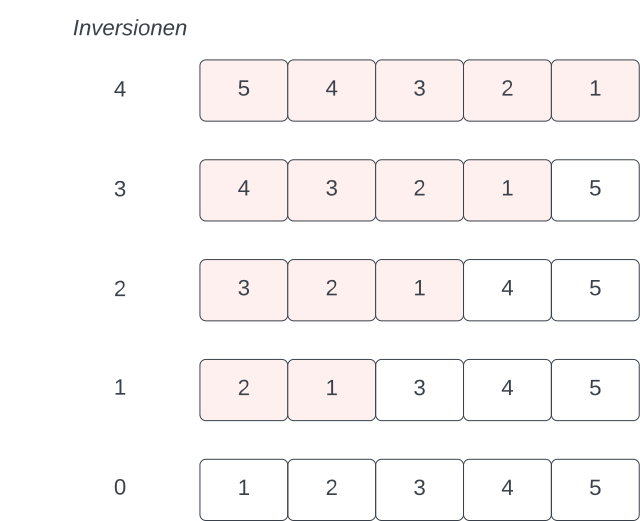
\includegraphics[scale=0.5]{chapters/Sortierverfahren/img/inversions}
        \caption{Fehlstellungen in einem absteigend sortierten Feld. (Quelle: eigene)}
        \label{fig:inversions}
    \end{center}
\end{figure}